\documentclass{beamer}
\usepackage[utf8]{inputenc}
\usepackage[UKenglish]{babel}
\usepackage[UKenglish]{isodate}
\usepackage{graphicx}
\usepackage{tikz}
\usepackage{phaistos}

\usetheme{Boadilla}
\beamertemplatenavigationsymbolsempty
\author{Paulius Dilkas}
\title{...}
%s\subtitle{}
\institute[]{School of Computing Science}
\date{12th September 2018}

\begin{document}
\maketitle

%\begin{frame}{Outline}
%  \tableofcontents
%\end{frame}

% TODO: mention probability, goal = 2, visited/unvisited

\begin{frame}{}
  \begin{figure}
    \centering
    
\begin{tikzpicture}[overlay]
      \only<1>{
        \fill[fill=black!20!white] (-1, -2) rectangle (2, 2);
        \fill[fill=black!20!white] (-2, -1) rectangle (-1, 2);
        \draw[step=1cm,very thin] (-2, -2) grid (2, 2);
        \node at (-1.5, -1.6) {\PHchild};
      }
      \only<2>{
        \fill[fill=black!20!white] (-1, -2) rectangle (2, 2);
        \fill[fill=black!20!white] (-2, 0) rectangle (-1, 2);
        \draw[step=1cm,very thin] (-2, -2) grid (2, 2);
        \node at (-1.5, -0.6) {\PHchild};
      }
      \only<3>{
        \fill[fill=black!20!white] (-1, -2) rectangle (2, 2);
        \fill[fill=black!20!white] (-2, 1) rectangle (-1, 2);
        \draw[step=1cm,very thin] (-2, -2) grid (2, 2);
        \node at (-1.4, 0.4) {\PHchild};
        \node at (-1.8, 0.4) {$\bigstar$};
      }
      \only<4>{
        \fill[fill=black!20!white] (-1, -2) rectangle (2, 2);
        \fill[fill=black!20!white] (-2, 1) rectangle (-1, 2);
        \draw[step=1cm,very thin] (-2, -2) grid (2, 2);
        \node at (-1.4, -0.6) {\PHchild};
        \node at (-1.8, -0.6) {$\bigstar$};
      }
      \only<5>{
        \fill[fill=black!20!white] (0, -2) rectangle (2, 2);
        \fill[fill=black!20!white] (-2, 1) rectangle (-1, 2);
        \fill[fill=black!20!white] (-1, 0) rectangle (0, 2);
        \fill[fill=black!20!white] (-1, -2) rectangle (0, -1);
        \draw[step=1cm,very thin] (-2, -2) grid (2, 2);
        \node at (-0.4, -0.6) {\PHchild};
        \node at (-0.8, -0.8) {$\bigstar$};
        \node at (-0.8, -0.5) {$\bigstar$};
      }
      \only<6>{
        \fill[fill=black!20!white] (0, -2) rectangle (2, 2);
        \fill[fill=black!20!white] (-2, 1) rectangle (-1, 2);
        \fill[fill=black!20!white] (-1, 0) rectangle (0, 2);
        \fill[fill=black!20!white] (-1, -2) rectangle (0, -1);
        \draw[step=1cm,very thin] (-2, -2) grid (2, 2);
        \node at (-1.4, -0.6) {\PHchild};
        \node at (-1.8, -0.8) {$\bigstar$};
        \node at (-1.8, -0.5) {$\bigstar$};
      }
      \only<7>{
        \fill[fill=black!20!white] (0, -2) rectangle (2, 2);
        \fill[fill=black!20!white] (-2, 1) rectangle (-1, 2);
        \fill[fill=black!20!white] (-1, 0) rectangle (0, 2);
        \fill[fill=black!20!white] (-1, -2) rectangle (0, -1);
        \draw[step=1cm,very thin] (-2, -2) grid (2, 2);
        \node at (-1.4, -1.6) {\PHchild};
        \node at (-1.8, -1.8) {$\bigstar$};
        \node at (-1.8, -1.5) {$\bigstar$};
      }
    \end{tikzpicture}
  \end{figure}
\end{frame}

\begin{frame}{A Tale of a Schr\"{o}dinger's Wall...}
  \begin{figure}
    \centering
    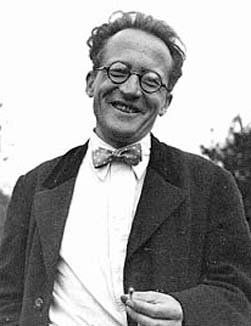
\includegraphics[height=\textheight]{schrodinger.jpg}
  \end{figure}
\end{frame}

% TODO: arrows for directions
\begin{frame}{}
  \begin{figure}
    \centering
    
\begin{tikzpicture}[overlay]
      \only<1>{
        % outside walls
        \draw (-0.25, 0.5) -- (-1.5, 0.5) -- (-1.5, 1.5) -- (1.5, 1.5) -- (1.5, 0.5) -- (0.25, 0.5);
        % background grid
        \draw[gray,very thin] (-0.5, 1.5) -- (-0.5, 0.5);
        \draw[gray,very thin] (0.5, 1.5) -- (0.5, 0.5);
        % agent
        \node at (-1, 0.9) {\PHchild};
        % door
        \draw[brown,ultra thick] (-0.25, 0.5) -- (0.25, 0.5);
      }
      \only<2>{
        % outside walls
        \draw (-0.25, 0.5) -- (-1.5, 0.5) -- (-1.5, 1.5) -- (1.5, 1.5) -- (1.5, 0.5) -- (0.25, 0.5);
        % background grid
        \draw[gray,very thin] (-0.5, 1.5) -- (-0.5, 0.5);
        \draw[gray,very thin] (0.5, 1.5) -- (0.5, 0.5);
        % agent
        \node at (0, 0.9) {\PHchild};
        % door
        \draw[brown,ultra thick] (-0.25, 0.5) -- (0.25, 0.5);
      }
      \only<3-4>{
        % outside walls
        \draw (1.5, 0.5) -- (1.5, -1.5) -- (-0.5, -1.5) -- (-0.5, 0.5) -- (-1.5, 0.5) -- (-1.5, 1.5) -- (1.5, 1.5) -- (1.5, 0.5) -- (0.5, 0.5);
        % probabilistic wall
        \draw[red,ultra thick,dashed] (0.5, 0.5) -- (0.5, -0.5);
        % background grid
        \draw[gray,very thin] (-0.5, 1.5) -- (-0.5, 0.5);
        \draw[gray,very thin] (0.5, 1.5) -- (0.5, 0.5);
        \draw[gray,very thin] (-0.5, -0.5) -- (1.5, -0.5);
        \draw[gray,very thin] (0.5, -0.5) -- (0.5, -1.5);
        % agent
        \node at (0, 0.9) {\PHchild};
        % door
        \draw[dotted] (-0.25, 0.5) arc (180:270:0.5cm);
        \draw[brown,ultra thick] (0.25, 0) -- (0.25, 0.5) node[right,  near start]{};
        \draw (-0.5, 0.5) -- (-0.25, 0.5);
        \draw (0.25, 0.5) -- (0.5, 0.5);
        % target
        \node at (1, 0) {$\bigstar$};
      }
      \only<4>{
        \draw[->, ultra thick, green] (0, 0.5) -- (0, 0) -- (0.8, 0);
        \draw[->, ultra thick, green] (0, 0.5) -- (0, -1) -- (1, -1) -- (1, -0.2);
      }
    \end{tikzpicture}
  \end{figure}
\end{frame}

\end{document}